\documentclass{standalone}
\usepackage{pgfplots}
\newcommand{\point}[2]{\pgfextractx{\dimen0}{\pgfpointanchor{#1}{#2}}\pgfextracty{\dimen2}{\pgfpointanchor{#1}{#2}}\typeout{POINT #1.#2: \the\dimen0,\the\dimen2}}
\newcommand{\report}{\point{current axis}{south west}\point{current axis}{north east}\point{current bounding box}{south west}\point{current bounding box}{north east}}
\newcommand{\labels}{\point{xl}{center}\point{xl}{text}\point{yl}{center}\point{yl}{text}}
\begin{document}
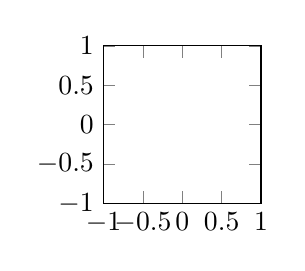
\begin{tikzpicture}
\begin{axis}[scale only axis,width=2cm,height=2cm,xmin=-1,xmax=1,ymin=-1,ymax=1]
\end{axis}
\typeout{CASE box}\report
\end{tikzpicture}
\begin{tikzpicture}
\begin{axis}[axis x line=middle,axis y line=middle,xmin=-1,xmax=6,ymin=-0.25,ymax=2.25,
  xlabel=$x$,ylabel=$y$,xlabel style={name=xl},ylabel style={name=yl}]
\end{axis}
\typeout{CASE middle}\report\labels
\end{tikzpicture}
\begin{tikzpicture}
\begin{axis}[axis x line=middle,axis y line=middle,xmin=-1,xmax=6,ymin=-0.25,ymax=2.25,
  xlabel=$x$,ylabel=$y$,enlargelimits=true,xlabel style={name=xl},ylabel style={name=yl}]
\end{axis}
\typeout{CASE enlarged}\report\labels
\end{tikzpicture}
\begin{tikzpicture}
\begin{axis}[axis x line=middle,axis y line=middle,xmin=1,xmax=2,ymin=3,ymax=4,
  xlabel=$x$,ylabel=$y$,enlargelimits=true,xlabel style={name=xl},ylabel style={name=yl}]
\end{axis}
\typeout{CASE positive}\report\labels
\end{tikzpicture}
\begin{tikzpicture}
\begin{axis}[width=16cm,height=8cm,axis x line=middle,axis y line=middle,
  xmin=-2,xmax=2,ymin=-1,ymax=2,ticks=none]
\end{axis}
\typeout{CASE tickless}\report
\end{tikzpicture}
\begin{tikzpicture}
\begin{axis}[width=16cm,height=8cm,axis x line=middle,axis y line=middle,
  xmin=-2,xmax=2,ymin=-1,ymax=2,xtick=\empty,ytick=\empty]
\end{axis}
\typeout{CASE tickless-empty}\report
\end{tikzpicture}
\begin{tikzpicture}
\begin{axis}[xmin=0,xmax=1,ymin=0,ymax=1,xtick={0},xticklabels={2012\\2956},
  tick label style={font=\footnotesize},xticklabel style={name=xt}]
\end{axis}
\typeout{CASE unaligned}\report\point{xt}{center}\point{xt}{text}\point{xt}{south west}\point{xt}{north east}
\end{tikzpicture}
\begin{tikzpicture}
\begin{axis}[xmin=0,xmax=1,ymin=0,ymax=1,xtick={0},xticklabels={2012\\2956},
  tick label style={font=\footnotesize,align=center},xticklabel style={name=xt}]
\end{axis}
\typeout{CASE aligned}\report\point{xt}{center}\point{xt}{text}\point{xt}{south west}\point{xt}{north east}
\end{tikzpicture}
\end{document}
